\section{Thesis environment}
\label{sec:thesis_env}

\subsection{\acs*{plat} project}
\label{subsec:platinum}
This thesis is founded by the French \Ac{anr} institute and is part of the \href{http://platinum.projets.litislab.fr/}{\ac{plat}} project (ANR-15-CE23-0010). \Ac{plat} is a long-term mapping project composed of three parts: high quality multi-sources map creation, online visual-based urban navigation with user feedback and automatic map update for long-life usage. The first part is an offline mapping step from multi-modal data sources collected by a mobile mapping vehicle~\citep{Paparoditis2012,Boussaha2018,Boussaha2018a} that produces a high resolution textured mesh with radiometric, geometric and semantic information. Then, this map is used as a reference for an online visual navigation module. During the navigation, an agent sends visual feedback to the server in order to, in a third step, update the map if changes are detected between the reference map and the current observation. The city center of Rouen, in France, have been chosen to carry out the project experiments.

The subject of this thesis is the initial localization of the agent over the entire map before the start of the navigation. We detail in the next paragraph the localization pipeline.

\subsection{The localization task}
\paragraph{Summary of the map.}
The online localization task within the \ac{plat} project consists of finding the position a visual data from the agent over a summarized version of the global map. To summarize the initial textured mesh, we render a set of radiometric (RGB), depth (D) and semantically labeled (L) spheres at meaningful location for covering the entire area of possible navigation~\citep{Salah2017, Salah2018, Salah2018a}. This representation contains all the modalities and most of the information from the original map while being much lighter.

\paragraph{Initial agent query.}
In order to start the visually-guided navigation of the agent, we have to find its absolute position on the mapped area. We assume that the agent is not equipped with any global localization equipment, such as GPS, and carry only an embedded device to acquire visual information. This is a regular assumption in urban area where global positional system can suffer from buildings obstruction (\eg the urban canyon effect that affects the GPS signal). In order to be globally located, the agent sends from his capture device a visual request to a server. By visual request, we regardless denote: monocular image, video sequence, pair of stereo images, semantically annotated image or combination of these.

\paragraph{Localization in a graph of spheres.}
Once the map has been summarized and the agent request received, the localization task can be compiled in this question: ``which RGBDL spheres is located closest to the agent visual query?''. In order to answer this question, we have to develop methods that can handle potentially multi-modal requests and compare them to augmented spherical images.

\begin{figure}[t]
	\centering

	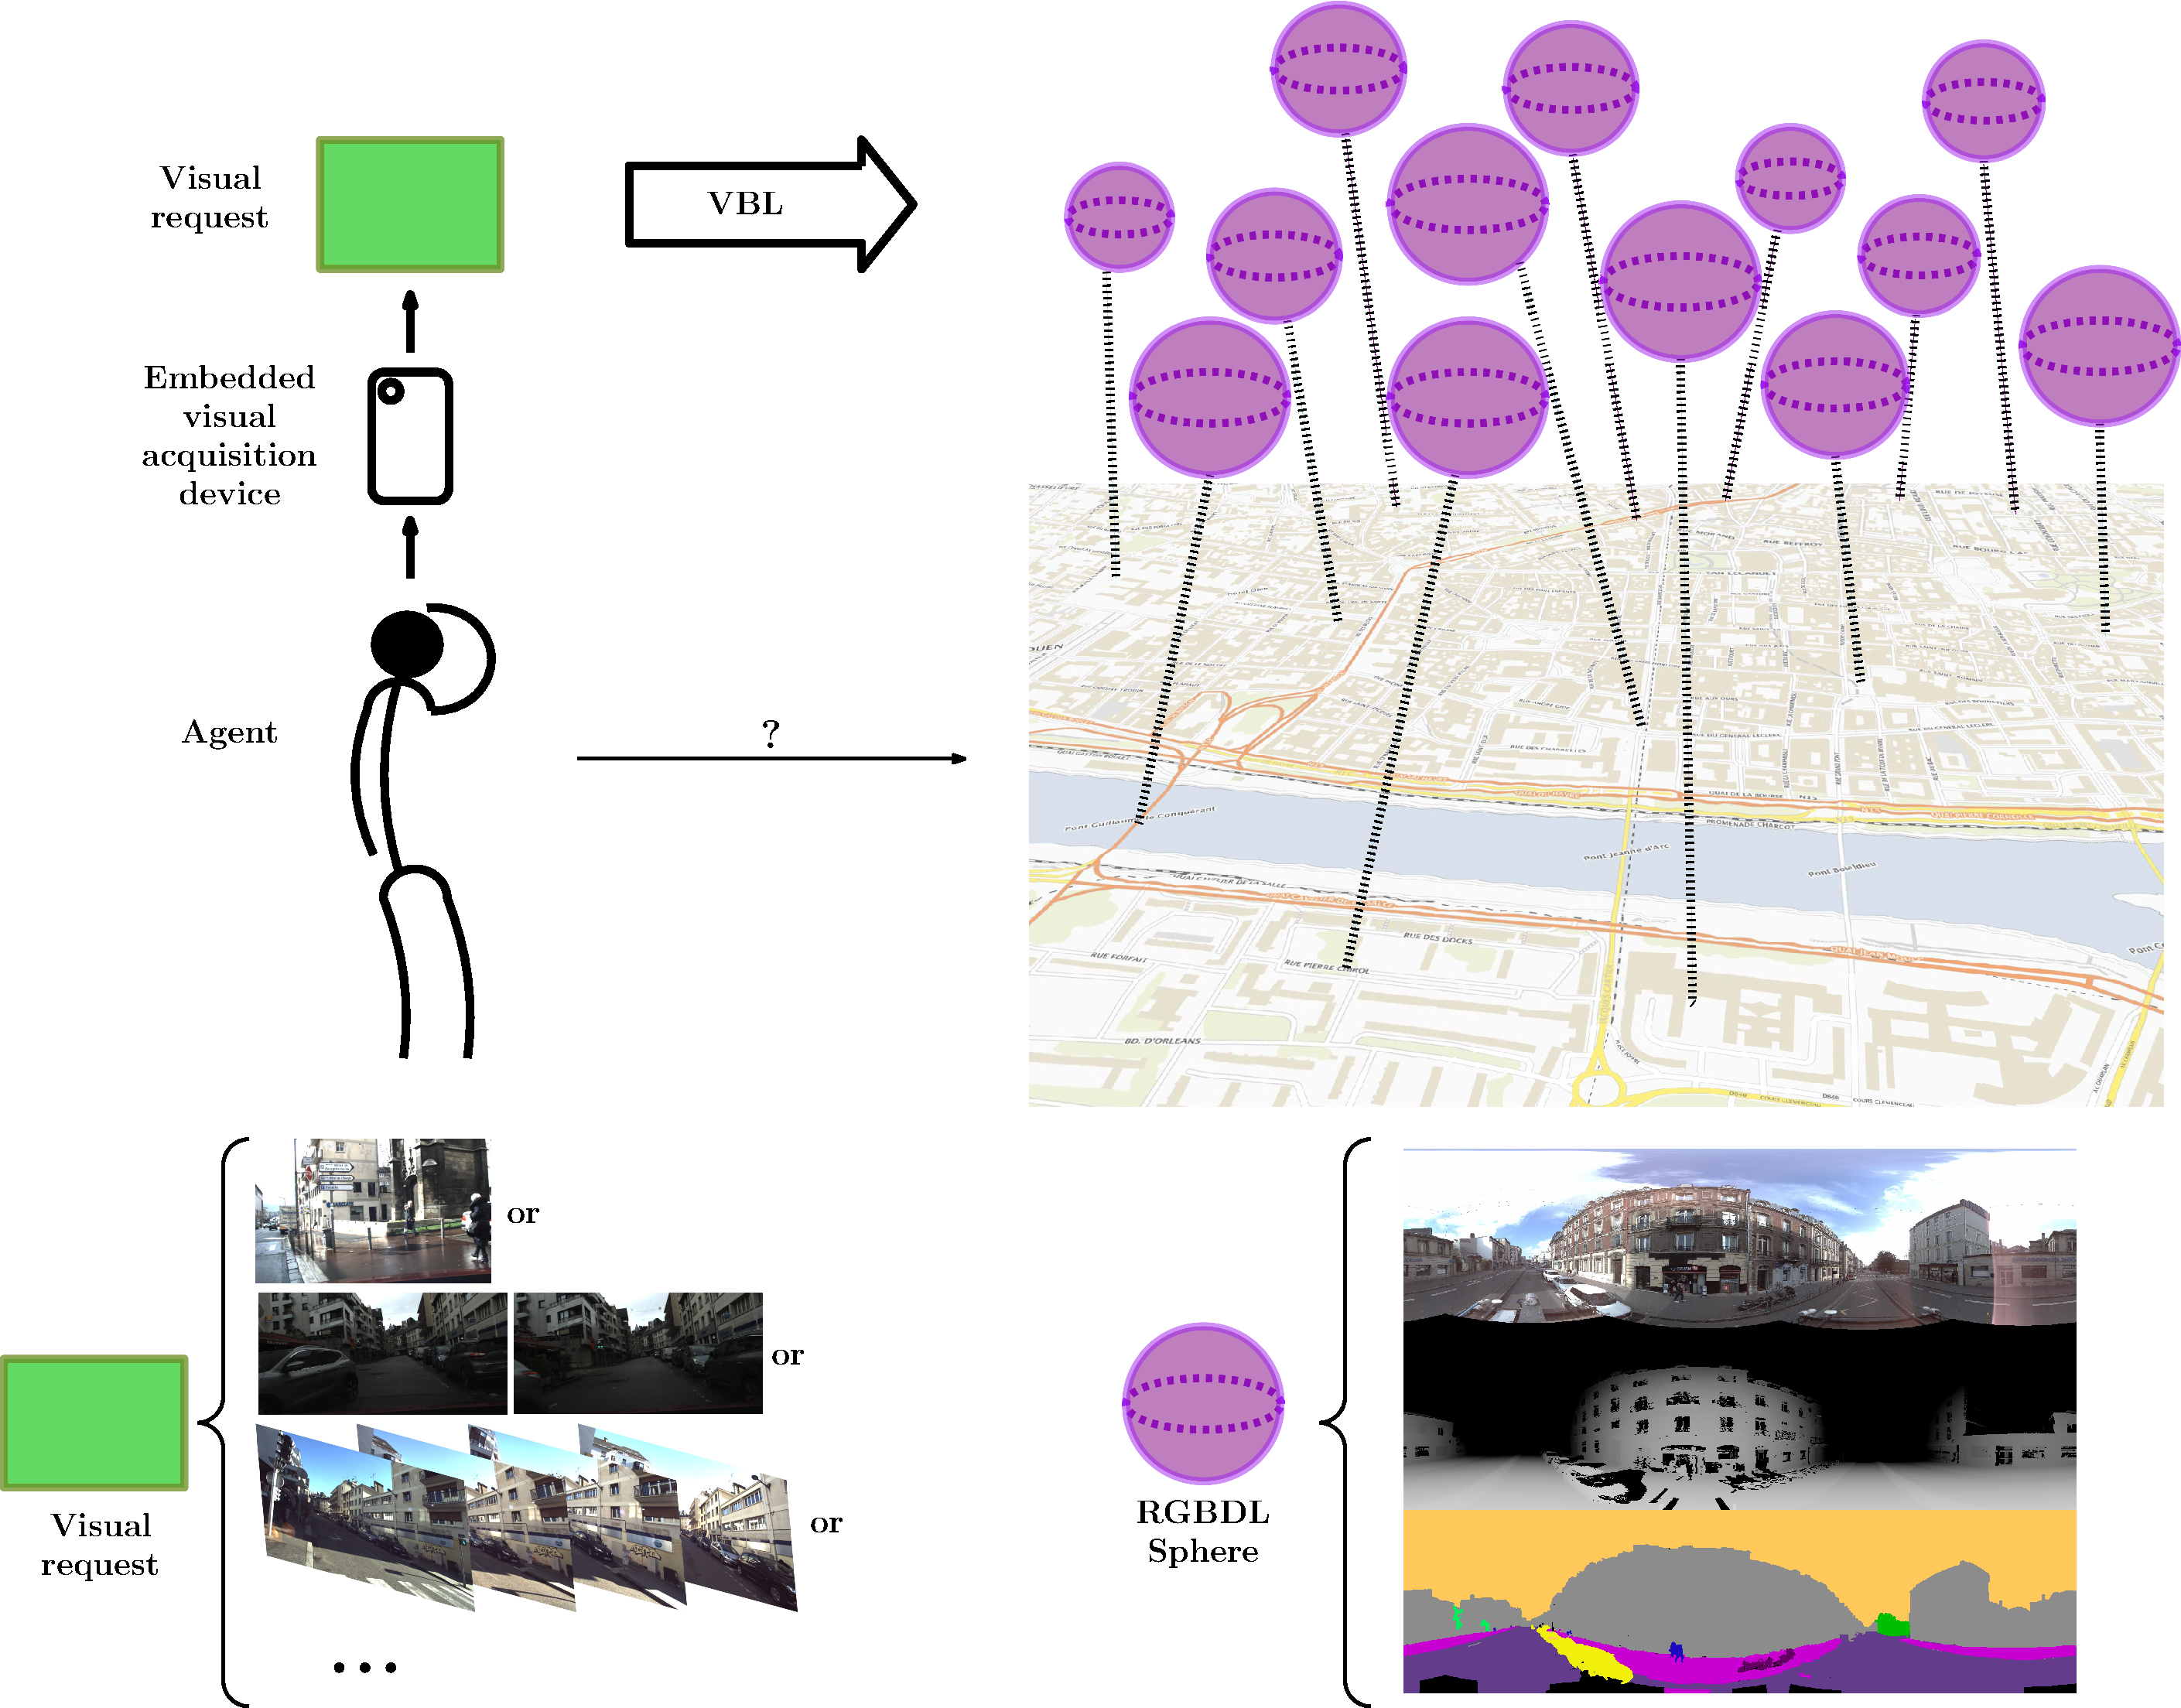
\includegraphics[width=\linewidth]{env/plat_resume}
	\caption[Localization task in \acs*{plat}]{\textbf{The localization task within the \acs*{plat} project:} \label{fig:plat_pipeline} }
\end{figure}


We present in figure~\ref{fig:plat_pipeline} the localization task considered within the \ac{plat} project.